\Aufgabe{Der Weg der Daten}{
    \begin{minipage}[t]{0.85\textwidth}
        \begin{enumerate}
            \item Öffne im Browser Orinoco: \UrlAndCode{klassenkarte.de/oo/} 
            \item Aus der linken Spalte benötigen wir die Elemente \emphColB{Eingabe, Funktion, Ausgabe und Datenfluss}.
            \item Wähle zwei verschiedene Formelfelder deiner Tabelle aus und erstelle ein Diagramm mit den genannten Elementen, das darstellt, welche Daten in die Berechnung einfließen, welche ausgegeben werden und was für eine Berechnung durchgeführt wird. 
            \item Erstellt möglichst viele Diagramme auf verschiedenen Abstraktionsebenen.
        \end{enumerate}
        
        \vspace{0.2cm}
        \Loesung{
            Ein paar Beispiele für eine Zelle. Es gibt natürlich seehr viele   Möglichkeiten.\\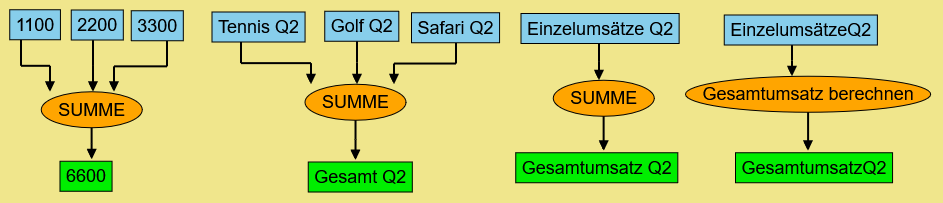
\includegraphics[width=\textwidth]{_Aufgaben/img/orinoo.png}
        }
    \end{minipage}
}